\PassOptionsToPackage{quiet}{xeCJK}
\documentclass[UTF8,a4paper]{ctexart}
\usepackage[text={165mm,245mm}]{geometry}
\usepackage{graphicx}
\usepackage{subfigure}
% \usepackage{ctex}
\usepackage{float} 
\usepackage{listings}
\usepackage{xcolor}
\usepackage{amsmath}
\usepackage{hyperref}
\usepackage{listings}
\newcommand{\code}{\texttt}
\graphicspath{{./img/}}
\definecolor{mygreen}{rgb}{0,0.6,0}  
\definecolor{mygray}{rgb}{0.5,0.5,0.5}  
\definecolor{mymauve}{rgb}{0.58,0,0.82}  


\title{\textbf{x-Eris 调研报告}}
\author{小组成员:胡天羽,罗胤玻,李润时,万辰希,吴书让}
\begin{document}
\maketitle

\section{项目概述}
\section{项目背景}
\subsection{嵌入式操作系统}
\subsubsection{概述}
\subsubsection{小结}

\subsection{非虚拟文件系统}
\subsubsection{概述}
\subsubsection{小结}

\subsection{虚拟文件系统 - Linux}
\subsubsection{概述}

虚拟文件系统(VFS)是操作系统中的一个抽象层,它允许不同的文件系统(例如
\href{https://en.wikipedia.org/wiki/Ext4}{ext4}、
\href{https://en.wikipedia.org/wiki/NTFS}{NTFS}
和
\href{https://en.wikipedia.org/wiki/File_Allocation_Table}{FAT32})
以一致的方式呈现其内容。虚拟文件系统为应用程序提供了一个通用的文件系统
API
接口,
亦可以用于透明地访问本地与网络存储设备而不让客户端应用程序察觉到差别。
它可以用来弥合
Windows, macOS,以及 Unix
的文件系统之间的差异,以便于应用程序访问这些不同类型的本地文件系统上的文件,
而无需得知其正在访问的文件系统类型。

虚拟文件系统规定了操作系统内核与具体文件系统之间的接口(或合同),
因此,只需满足这些借口所需的条件即可向内核添加对新文件系统的支持。
但是,这些文件接口所需要满足的条件可能随着操作系统版本的更新而发生变化,
这便会要求对某一具体文件系统的支持程序进行一定的修改,
并且重新编译操作系统内核。当然,操作系统的开发者也可以选择向后兼容的更新改版,
使之前版本的具体文件系统支持程序继续工作在更新后的操作系统上。

\begin{figure}[H]
    \centering
    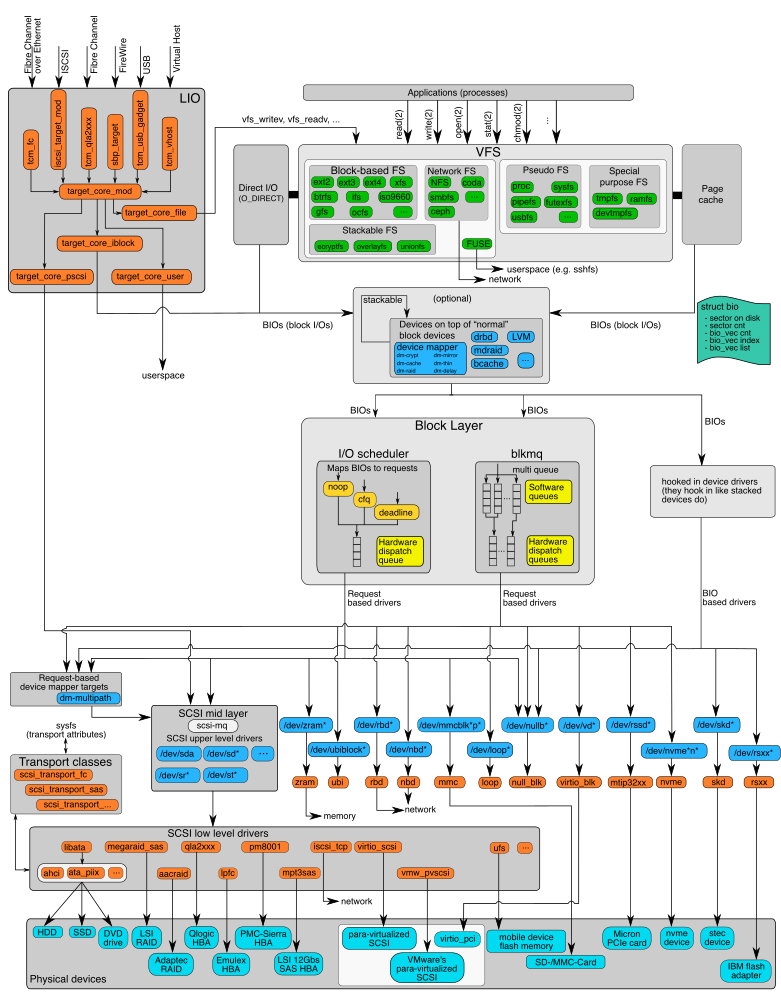
\includegraphics[width=0.6\textwidth]{The_Linux_Storage_Stack_Diagram.png}
    \caption{The Linux Storage Stack Diagram}
\end{figure}

上图为 VFS 层在 Linux 内核存储栈中相对各个部分的位置。

Linux文件系统的灵活性和可扩展性是抽象接口集的直接结果。
这个接口集的核心是便虚拟文件系统开关(VFS)。

VFS为上层应用程序提供一组标准接口,
以便在多种文件系统上执行文件读写,
并支持在一个或多个底层设备上同时使用多个文件系统。
此外,这些文件系统并不需要是静态的,它们可能会随着存储设备的瞬态性而改变。
例如,一个典型的
Linux 桌面系统支持可用硬盘上的 ext3 文件系统,以及可用
\href{https://en.wikipedia.org/wiki/CD-ROM}{CD-ROM} 上的
\href{https://en.wikipedia.org/wiki/ISO_9660}{ISO 9660} 
文件系统(也称为
CD-ROM 文件系统或 CDFS)。
随着 CD-ROM 的插入和移除,Linux
内核必须适应这些具有不同内容和结构的新文件系统。
远程文件系统可以通过网络文件系统(NFS)访问。同时,Linux
可以从本地硬盘上的 Windows/Linux 双启动系统中挂载 NT
文件系统(NTFS)分区,并从中读取和写入数据。

同样,可移动的 USB
闪存驱动器(UFD)可以热插拔,提供另一个文件系统。
在此期间,这些相同的文件接口,允许将底层文件系统和物理设备抽象出来,
以便用户使用,见下图。

\begin{figure}[H]
    \centering
    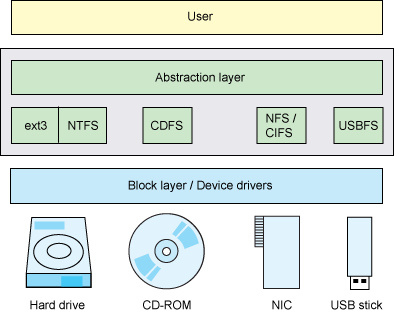
\includegraphics[width=0.4\textwidth]{figure1.jpg}
    \caption{文件系统和物理设备}
\end{figure}

\subsubsection{Layer Abstraction}

\begin{figure}[H]
    \centering
    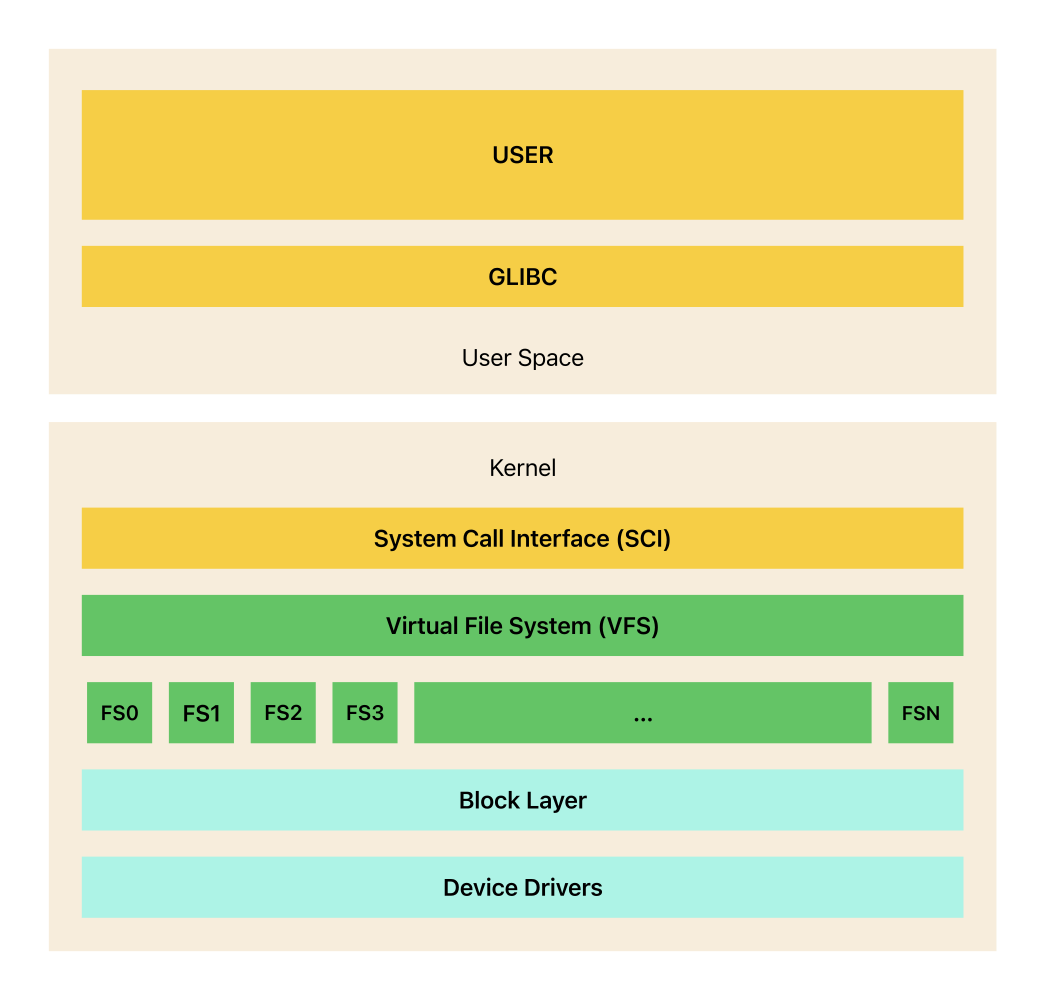
\includegraphics[width=0.6\textwidth]{The layered architecture of the VFS.png}
    \caption{The layered architecture of the VFS}
\end{figure}

接下来,对 Linux VFS 提供的抽象特性添加一些具体的架构。上图展示了从 VFS
的角度看 Linux 栈的高层视图。在 VFS
的上方是标准内核系统调用接口
(\href{https://en.wikipedia.org/wiki/Scalable_Coherent_Interface}{SCI})。
这个接口允许用户空间的调用从不同的地址空间过渡到内核中。
在这个域中,一个用户空间应用程序激发
\href{https://en.wikipedia.org/wiki/POSIX}{POSIX} open call 通过
\href{https://en.wikipedia.org/wiki/GNU}{GNU} C
库(\href{https://en.wikipedia.org/wiki/Glibc}{glibc})
进入内核并进入系统调用解多路器。最终,使用
\code{sys\_open} 调用 VFS。

VFS 提供抽象层,
将 POSIX API
与特定文件系统实现该行为的细节分离。
关键在于,
无论底层文件系统是
ext3还是Btrfs,
打开,
读取,
写入或关闭的 API
系统调用都是相同的。
VFS提供了一个底层文件系统可以继承的共同文件模型
(它们必须能够实现各种
POSIX API
的函数)。
在VFS之外,
还有一个抽象层将底层物理设备隐藏起来,
这些底层物理设备可以是是磁盘、
磁盘分区、
网络存储实体、
内存或任何能够存储信息,
甚至是短暂存储介质。

除了将底层文件操作与可用文件系统联系起来,
VFS还将底层块设备与可用文件系统联系起来。

\subsubsection{Superblock}

Superblock 是一个关于文件系统高级元数据的容器。
Superblock
是一个存在于磁盘(实际上是多个位置上的冗余信息)
和内存中的结构。它是处理磁盘上文件系统的基础,
因为它定义了文件系统的管理参数,例如,总块数、可用块数、根索引节点。

在磁盘上,superblock
向内核提供有关磁盘上文件系统结构的信息。
在内存中,superblock
提供了管理已挂载文件系统所需的信息和状态。因为 Linux
支持在同一时间挂载多个并发文件系统,所以每个 \texttt{super\_block}
结构都在一个 \texttt{super\_blocks} 列表中维护(\texttt{super\_blocks}
在 \texttt{./linux/fs/super.c} 中定义,\texttt{super\_block}结构在
\texttt{/linux/include/fs/fs.h} 中定义)。

\begin{figure}[H]
    \centering
    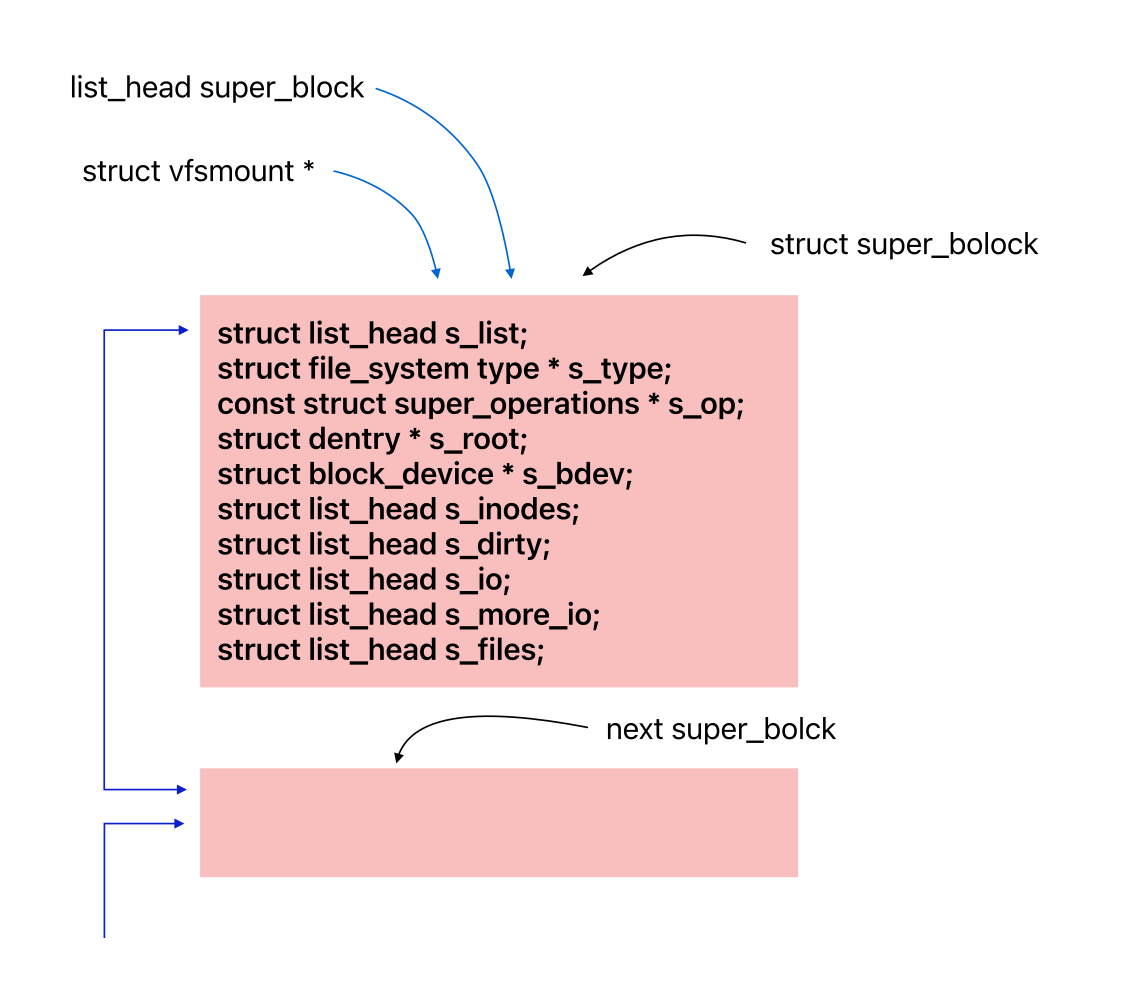
\includegraphics[width=0.6\textwidth]{Simplified view of the super_block structure and its related elements.png}
    \caption{Simplified view of the super\_block structure and its related elements}
\end{figure}

上图为 superblock 及其元素的简化视图。\texttt{super\_block}
结构引用了许多封装其他信息的结构体。例如,\texttt{file\_system\_type}
结构体维护文件系统的名称(如ext3)以及获取和删除 \texttt{super\_block}
的各种锁和函数。\texttt{file\_system\_type}
对象通过著名的\texttt{register\_file\ system} 和
\texttt{unregister\_file\ system} 函数进行管理(见
\texttt{./linux/fs/file\ systems.c})。\texttt{super\_operations}
结构定义了读写索引节点以及更高级别操作的多个函数,如重新挂载。
根目录条目(dentry)对象与此文件系统所在的块设备同样在此被缓存。最后,superblock
提供多个列表来管理索引节点,包括
\texttt{s\_inodes}(所有索引节点的列表)、
\texttt{s\_dirty}
(所有脏索引节点的列表)、\texttt{s\_io}
和
\texttt{s\_more\_io}(停止进行写回)、
\texttt{s\_files}(给定文件系统的所有打开文件的列表)。

另外,Linux 内核中还有另一个管理对象称为
\texttt{vfsmount},它提供有关挂载的文件系统的信息。这些对象的列表引用了
superblock 并定义了挂载点,文件系统所在的 \texttt{/dev}
设备的名称,以及其他更高级别的附加信息。


\subsubsection{The Index Node (inode)}
Linux 通过一个称为
inode(索引节点)的对象来管理文件系统中的所有对象。一个 inode
可以指向一个文件、一个目录或另一个对象的符号链接。因为文件用于表示其他类型的对象比如设备或内存,inode
也用于表示它们。

请注意,这里提到的 inode 是 VFS 层的 inode(内存
inode)。事实上,每个文件系统还包括一个
inode,它位于磁盘上,能够提供有关特定文件系统对象的详细信息。

VFS inode 使用
slab分配器(来自 \texttt{inode\_cache})进行分配。其由描述 inode
与内容以及可能在 inode 上执行的各种操作的数据和操作组成。

\begin{lstlisting}[language=C]
struct list_head i_dentry;
struct timespec i_atime;
struct timespec i_mtime;
struct timespec i_ctime;
gid_t i_gid;
uid_t i_uid;
loff_t i_size;
const struct file_operations * i_fop;
const struct inode_operations * i_op;
struct address_space * i_maping;
struct address_space * i_data;
…
\end{lstlisting}

以上是一个简单的 VFS inode 示例,包含多个列表,其中一个列表引用了指向此
inode 的
dentries。对象级元数据包括熟悉的操作时间(创建时间、访问时间、修改时间),以及所有者和权限数据(group-id、user-ID
和 permissions)。inode
引用了可能在其上执行的文件操作,其中大多数直接映射到系统调用接口(例如,\texttt{open}、\texttt{read}、\texttt{write}
和 \texttt{flush})。还有一个引用 inode 特定操作的结构(如
\texttt{create}、\texttt{lookup}、\texttt{link}、\texttt{mkdir}
等)。最后,还有一个结构来管理由地址空间对象表示的对象的实际数据。\texttt{address\ space}
对象是一个管理 inode
在页面缓存中的各个页面的对象。地址空间对象用于管理文件的页面,并将文件段映射到各个进程地址空间中。地址空间对象配有自己的操作集(\texttt{writepage}、\texttt{readpage}、\texttt{releasepage}
等)。

\subsubsection{Directory Entry (dentry)}

Linux 中的另一个对象,称为 \texttt{dentry}
对象,它用于管理文件系统的分层结构。文件系统有一个根 dentry(在
\texttt{super\_block} 中被引用),这是唯一一个没有 parent 的
dentry。所有其他 dentry 都有 parent,有些有 children。例如,如果打开了由
\texttt{/home/user/name} 组成的文件,则将会有四个 dentry
对象被创建:一个用于根目录 \texttt{/},一个用于根目录的 \texttt{home}
条目,一个用于 \texttt{user} 目录的 \texttt{name} 条目,最后,一个用于
\texttt{user} 目录的 \texttt{name} 条目的
\texttt{dentry}。通过这种方式,dentry
在今天使用的分层文件系统中拥有非常清晰的映射。

dentry 对象由 \texttt{dentry} 结构(位于
\texttt{./linux/include/fs/dcache.h})定义。
它包括一些用于跟踪该条目与文件系统中其他条目关系,
以及物理数据(例如文件名)的元素。

\begin{lstlisting}[language=C]
struct wuper_block * d_sb;
struct dentry * d_parent;
struct list_head d_subdirs;
struct dentry_operations * d_op;
unsigned char d_iname[];
struct inod * d_inode;
…
\end{lstlisting}

以上展示了 dentry 对象的简化视图。dentry 引用了 super\_block,而
\texttt{super\_block}
定义了包含该对象的特定文件系统实例。接下来是该对象的 parent
dentry(父目录),后跟包含在列表中的 child
dentry(如果该对象恰好是目录),然后定义了 dentry 的操作(包括
\texttt{hash},\texttt{compare},\texttt{delete},\texttt{release}
等操作)。对象的名称随后被定义,该名称在 dentry 中而不是 inode
本身中保存。最后,提供了对VFS inode的引用。

请注意,dentry
对象仅存在于文件系统内存中,不会存储在磁盘上。只有文件系统 inode
被永久存储,而 dentry
对象用于提高性能。可以在\texttt{./linux/include/dcache.h} 中查看 dentry

\subsubsection*{File Object}

对于 Linux
系统中每个打开的文件,都存在一个文件对象。
该对象包含给定用户的打开实例的相关信息。
文件对象的一个较为简化的视图下面中提供。

\begin{lstlisting}[language=C]
struct path    f_path;
struct dentry (f_path, dentry);
const struct file_operations * f_op;
unsigned int f_flags;
fmode_t f_mode;
lodd_t f_ops;
…
\end{lstlisting}

如图所示,路径结构提供了对 dentry 和 vfsmount
的引用。为每个文件定义了一组文件操作,
这些操作是众所周知的文件操作(例如打开、关闭、读取、写入、刷新等)。
还定义了一组标志和权限(包括组和所有者)。
最后,为特定的文件实例定义了有状态数据,
例如文件的当前偏移量。
\subsubsection{小结}
VFS(虚拟文件系统)
是 Linux
内核中的一个抽象层,它提供了一组标准的文件系统操作,这些操作可以在不同的文件系统上实现。
VFS
的内部架构由一个提供文件系统抽象的分派层和一些缓存组,
以此能够提高文件系统操作的性能。

\begin{figure}[H]
    \centering
    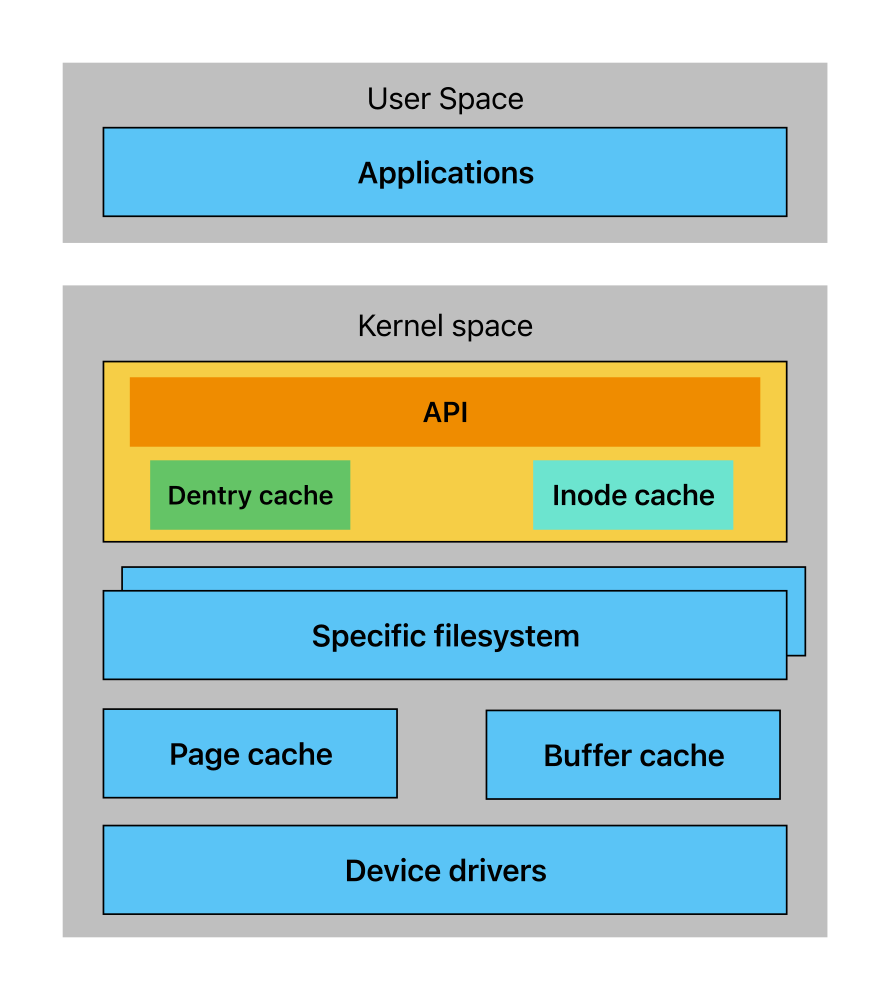
\includegraphics[width=0.6\textwidth]{High-level view of the VFS layer.png}
    \caption{VFS 层的高级视图}
\end{figure}

在 VFS 中,两个主要的动态管理对象包括 \texttt{dentry} 和 \texttt{inode}
对象。将这些对象缓存可以提高对底层文件系统的访问性能。当打开一个文件时,\texttt{dentry}
缓存将被填充以表示路径所代表的目录级别的条目。同时还会创建一个 inode
表示文件的对象。\texttt{dentry}
缓存使用哈希表构建,由对象名称进行哈希。\texttt{dentry} 缓存的条目是从
\texttt{dentry\_cache} 的 slab
分配器中分配的,并使用最近最少使用(\href{https://en.wikipedia.org/wiki/Cache_replacement_policies\#LRU}{LRU})
算法来修剪条目以应对内存压力。与
\texttt{dentry} 缓存相关的函数可以在 \texttt{./linux/fs/dcache.c}和
\texttt{./linux/include/linux/dcache.h} 中找到。

\texttt{inode}
缓存是由两个列表和一个哈希表实现的,这样可以实现更快地查找。第一个列表定义了当前正在使用的
\texttt{inodes},第二个列表定义了未使用的 \texttt{inodes}。正在使用的
\texttt{inodes} 也存储在哈希表中。从 \texttt{inode\_cache} 的 slab
分配器中分配单个 \texttt{inode} 缓存对象。与 \texttt{inode}
缓存相关的函数可以在\texttt{./linux/fs/inode.c} 与
\texttt{./linux/include/fs.h} 中找到。

从实现来看,\texttt{dentry} 缓存是 \texttt{inode} 缓存的主控制器。当
\texttt{dentry} 对象存在时,\texttt{inode} 对象也会存在于 \texttt{inode}
缓存中。在 \texttt{dentry} 缓存上执行查找,将导致在 \texttt{inode}
缓存中获得一个对象。

\subsection{虚拟文件系统 - 嵌入式}
\subsubsection{概述}
本部分主要介绍了 \texttt{FreeRTOS-Plus-FAT} 以及 \texttt{RT-Thread} 
中的文件系统实现细节。

在早期的嵌入式系统中,需要存储的数据比较少,
数据类型也比较单一,往往使用直接在存储设备中的指定地址写入数据的方法来存储数据。
然而随着嵌入式设备功能的发展,需要存储的数据越来越多,也越来越复杂,
这时仍使用旧方法来存储并管理数据就变得非常繁琐困难。
因此需要新的数据管理方式来简化存储数据的组织形式,需要新的文件系统设计。

\subsubsection{\texttt{FreeRTOS-Plus—FAT}}
通过阅读源代码,可以简单分类此项目的文件组织如下。
\begin{itemize}
\item 主要
\begin{itemize}
    \item \texttt{ff\_dir}: 用于访问文件夹中内容
    \item \texttt{ff\_fat}: 用于访问 \texttt{FAT} 文件系统
    \item \texttt{ff\_file}: 用于文件读写
    \item \texttt{ff\_ioman}: 管理缓存和挂载读写对象(介质)
    \item \texttt{ff\_format}: 格式化或分区介质
    \item \texttt{ff\_locking}: 加锁?
    \item \texttt{ff\_memory}: 从内存读取数据
    \item \texttt{ff\_stdio}: 用于文件管理(统计),相对路径转换
    \item \texttt{ff\_sys}: 用于映射文件系统到根目录
\end{itemize}
\item 辅助
\begin{itemize}
    \item \texttt{ff\_headers}: 管理所有头文件
    \item \texttt{ff\_time}: 获取时间
    \item \texttt{ff\_error}:  用于错误处理
    \item \texttt{ff\_crc}: 用于计算 \texttt{CRC}(循环检验码)
    \item \texttt{ff\_string}: 字符串库
\end{itemize}
\item 驱动
\begin{itemize}
    \item 各处理器相应的文件系统驱动
\end{itemize}
\end{itemize}

\paragraph{\texttt{ERRNO} 值} \texttt{FreeRTOS-Plus-FAT} 文件系统的标准 API 与标准 C 库使用相同的 \texttt{errno} 值。
标准 C 库中的文件相关函数返回 0 表示通过,返回 -1 则表示失败。如果返回 -1,则失败的原因 存储在名为 \texttt{errno} 的变量中,须单独检查。 
同样,\texttt{FreeRTOS-Plus-FAT} 的标准 API 返回 0 表示通过,返回 -1 则表示失败, 该 \texttt{API} 还会针对各项 \texttt{RTOS} 任务维护 \texttt{errno} 变量。

\subsubsection{\texttt{RT-Thread}}
此文件系统有较多简介,可供设计参考,它的特点是:
\begin{itemize}
    \item 为应用程序提供统一的 \texttt{POSIX} 文件和目录操作接口:\texttt{read}、\texttt{write}、\texttt{poll/select} 等。
    \item 支持多种类型的文件系统,如 \texttt{FatFS}、\texttt{RomFS}、\texttt{DevFS} 等,并提供普通文件、设备文件、网络文件描述符的管理。
    \item 支持多种类型的存储设备,如 \texttt{SD Card}、\texttt{SPI Flash}、\texttt{Nand Flash} 等。
\end{itemize}
\paragraph{POSIX 文件系统接口}

\texttt{POSIX} 表示可移植操作系统接口,\texttt{POSIX} 标准定义了操作系统应该为应用程序提供的接口标准,是 \texttt{IEEE} 为要在各种 \texttt{UNIX} 操作系统上运行的软件而定义的一系列 \texttt{API} 标准的总称。

此标准意在期望获得源代码级别的软件可移植性。换句话说,为一个 \texttt{POSIX} 兼容的操作系统编写的程序,应该可以在任何其它 \texttt{POSIX} 操作系统(即使是来自另一个厂商)上编译执行。\texttt{RT-Thread} 支持 \texttt{POSIX} 标准接口,因此可以很方便的将 Linux/Unix 的程序移植到 RT-Thread 操作系统上。

\paragraph{虚拟文件系统层}
用户可以将具体的文件系统注册到 \texttt{DFS} 中,如 \texttt{FatFS}、\texttt{RomFS}、\texttt{DevFS} 等,具体介绍请参考其他小节。

\paragraph{设备抽象层}
设备抽象层将物理设备如 \texttt{SD Card}、\texttt{SPI Flash}、\texttt{Nand Flash},抽象成符合文件系统能够访问的设备,例如 \texttt{FAT} 文件系统要求存储设备必须是块设备类型。

不同文件系统类型是独立于存储设备驱动而实现的,因此把底层存储设备的驱动接口和文件系统对接起来之后,才可以正确地使用文件系统功能。
\subsubsection{小结}
设计 \texttt{VFS} 时,可以参考 \texttt{RT-Thread} 的三层结构组织形式、\texttt{FreeRTOS-Plus-FAT} 的API函数设计理念,将 \texttt{FreeRTOS-Plus-FAT} 继续拓展优化。

例如,可通过以下几点提高\textbf{兼容性}。(利用 \texttt{POSIX} 文件系统接口和与 \texttt{FreeRTOS-Plus-POSIX} 的结合将有可能方便地运行从 \texttt{Linux/Unix} 上移植的程序。
虽然目前 \texttt{FreeRTOS-Plus-POSIX} 对 \texttt{POSIX API} 的支持还不够充分,但是随着开发实用价值将逐渐上升。)

\begin{itemize}
    \item 继续采用标准 \texttt{eerno} 值
    \item 添加 \texttt{POSIX} 文件系统接口
    \item 添加支持的文件系统(磁盘文件系统、闪存文件系统)
    \item 拓展支持的实用函数
\end{itemize}

\subsection{文件系统开发}
\subsubsection{概述}
\subsubsection{小结}

\section{立项依据}

%\begin{figure}[H]
%    \centering
%    \includegraphics[scale=0.37]{p1.jpg}
%    \caption{图1}
%\end{figure}


\section{前瞻性/重要性分析}
\subsection{...}
\section{相关工作}
\subsection{\href{https://www.freertos.org/zh-cn-cmn-s/FreeRTOS-Plus/FreeRTOS_Plus_FAT/index.html}{FreeRTOS-Plus-FAT}}
是本项目的基础,主要使用 C语言 写成。源代码组织简洁,内容完整。但没有文档支持,建议直接阅读代码。
其主要可借鉴特性:
\begin{itemize}
    \item 采用标准 eerno 值
    \item 项目结构组织清晰
\end{itemize}
\subsection{\href{https://www.rt-thread.org/document/site/\#/rt-thread-version/rt-thread-standard/programming-manual/filesystem/filesystem}{RT-Thread/DFS}}
是RT-Thread的虚拟文件系统实现,文档详尽,可与上一个项目结合理解虚拟文件系统的一些设计理念。
其主要可借鉴特性:
\begin{itemize}
    \item 采用 POSIX 接口
    \item 目录管理相关使用函数较多
    \item 有关于文件系统配置方面参数的介绍
\end{itemize}

\subsection{相关工作二}
\subsection{相关工作三}
\subsection{相关工作四}
\subsection{相关工作五}

\section{参考资料}
\begin{enumerate}
    \item 
    
\end{enumerate}
\end{document}